\documentclass{article}
\setlength{\parskip}{0pt} % esp. entre parrafos
\setlength{\parindent}{20pt} % esp. al inicio de un parrafo
\usepackage{amsmath} % mates
\usepackage{listings}
\usepackage{xcolor}
\usepackage[sort&compress,numbers]{natbib} % referencias
\usepackage{url} % que las URLs se vean lindos
\usepackage[top=10mm,left=20mm,right=20mm,bottom=25mm]{geometry} % \textbf{\textbf{}}margenes
\usepackage{hyperref} % ligas de URLs
\usepackage{graphicx} % poner figuras
\usepackage{caption}
\usepackage{subcaption}
\usepackage[spanish]{babel} % otros idiomas
\hypersetup{
    colorlinks=true,
    linkcolor=blue,
    filecolor=blue,      
    urlcolor=blue,
}
\renewcommand{\lstlistingname}{Código}
\definecolor{codeblack}{rgb}{0,0.6,0}
\definecolor{codegray}{rgb}{0.5,0.5,0.5}
\definecolor{codepurple}{rgb}{0.58,0,0.82}
\definecolor{backcolour}{rgb}{0.95,0.95,0.92}
\lstdefinestyle{mystyle}{
    backgroundcolor=\color{backcolour},   
    commentstyle=\color{codeblack},
    keywordstyle=\color{blue},
    numberstyle=\tiny\color{codegray},
    stringstyle=\color{codeblack},
    basicstyle=\ttfamily\footnotesize,
    breakatwhitespace=false,         
    breaklines=true,                 
    keepspaces=true,                 
    numbers=left,                    
    numbersep=5pt,                  
    showspaces=false,                
    showstringspaces=false,
    showtabs=false,                  
    tabsize=2
}
\lstset{style=mystyle}

\title{"P7" Búsqueda Local}
\author{NESTOR}
\date {Marzo 2022}

\begin{document}

\maketitle

\section{Objetivo}\label{obj}
El objetivo de la práctica consiste en una variante unidimensional, a partir de un punto seleccionado al azar. Los movimientos locales, por medio de una búsqueda local aleatoria con restricciones en los ejes. Se realizarán  réplicas, y el menor de ellos es el resultado de la búsqueda en sí. \cite{elisa1}

\section{Desarrollo}\label{des}
Basando el desarrollo en la \href{https://github.com/satuelisa/Simulation/blob/master/LocalSearch/minimize1D.py}{codificación} implementado por E. Schaeffer \cite{elisa1} y se encuentra todas las instrucciones en el repositorio \href{https://github.com/NestorZeus/SIMULACION-COMPUTACIONAL-DE-NANOMATERIALES/tree/main/Phttps://github.com/NestorZeus/SIMULACION-COMPUTACIONAL-DE-NANOMATERIALES/tree/main/P7}{repositorio} de Nestor en GitHub.\\

Para comenzar se hace primero generar la función para graficar con los límites y los pasos.  \href{https://github.com/satuelisa/Simulation/blob/master/LocalSearch/minimize1D.py} implementados por E. Schaeffer, como se muestra a continuación en el código.

\begin{lstlisting}[caption=Generamos la función, language=Python]
import numpy as np
import math as ma
from matplotlib import cm
from mpl_toolkits.mplot3d import Axes3D
def g(x, y):
 return (1 - x/2 + x**5 + y**3) * np.exp(-x**2 - y**2)
 low = -2.7
 high = -low
 step = 0.10
\end{lstlisting}

Posteriormente generaramos cuantos son los que queremos de los puntos ó muestras con los ciclos ó pasos. Para esta práctica se usará 5 puntos ó muestras con 500 ciclos ó pasos con las posiciones. al tener las celdas se crea generar el cuadro con las funciones que es como inicia el programa como vemos en el código \ref{codigo2}.

\begin{lstlisting}[caption=Generamos los puntos ó muestras y los ciclos ó pasos, label=codigo2, language=Python]
puntos= 5
ciclos= 500
posx = [uniform(low, high) for s in range(puntos)]
posy = [uniform(low, high)for s in range(puntos)]
bestx = posx
besty = posy
\end{lstlisting}

Se realiza un ciclo for con la funcion movimientos para las posiciones, se muestra a continuación en el código \ref{codigo3}. Ya que esto nos muestra que en cada punto va a revisar sus vecinos y va a tomar la mejor posición, por cada punto revisa la posición y revisa sus vecinos y si hay un vecino más grande de mejor posición ese será la nueva posición.

\begin{lstlisting}[caption=Ejecución de códigos para los vecinos y posiciones, label=codigo3, language=Python]
def vecinos(vecindad):
    pos=[]
    for a in vecindad:
        pos.append((g(a[0],a[1]),a[0],a[1]))
    return(pos)
    
def movimientos(x, y, bx, by):
  pasos=[]
  listax,listay=[],[]
  listamxy=[]
    for s in range(puntos):
    mejorx,mejory=bx[0],by[0]
    cx, cy= x[s], y[s]
    Dx=uniform(0, step/3)
    Dy=uniform(0, step/3)
    xi, xd= (cx-Dx), (cx+Dx)
    yi, yd= (cy-Dy), (cy+Dy)
    xi = low if xi < low else xi
    xd = high if xd > high else xd
    yi = low if yi < low else yi
    yd = high if yd > high else yd
    vecindad=[(xi,yd),(cx,yd),(xd,yd),(xi,cy),(xd,cy),(xi,yi),(cx,yi),(xd,yi)]
    datos=vecinos(vecindad)
    pos,cx,cy= (max(datos))
    if pos > g(mejorx,mejory):
    mejorx, mejory=cx,cy
    else:
    mejorx, mejory= bx[0], by[0]
\end{lstlisting}

\section{Resultados}\label{res}

El eje horizontal representa los valores de las $x$, mientras que el eje vertical representa los valores de las $y$. Cada uno de los puntos rojos que se observan es un agente que realiza un movimiento, $\Delta x$ y $\Delta y$ cuyas combinaciones se hacen las posiciones. 

\begin{figure}
    \centering
    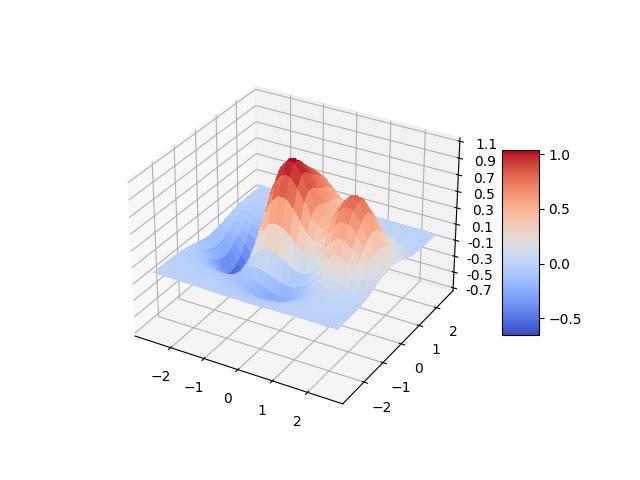
\includegraphics[width=200mm]{Figure_1.png}
    \caption{Diagrama en tres dimensiones.}
    \label{figure}
\end{figure}
\newpage
\begin{figure}
     \centering
     \begin{subfigure}[b]{0.40\textwidth}
         \centering
         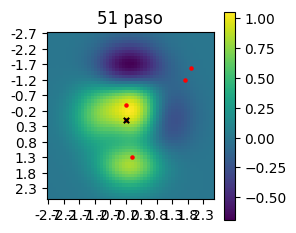
\includegraphics[width=\textwidth]{p7p_50.png}
         \caption{}
         \label{fig:notocan}
     \end{subfigure}
     \begin{subfigure}[b]{0.40\textwidth}
         \centering
         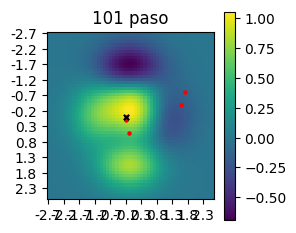
\includegraphics[width=\textwidth]{p7p_100.png}
         \caption{}
         \label{fig:tocan}
     \end{subfigure}
     \begin{subfigure}[b]{0.40\textwidth}
         \centering
         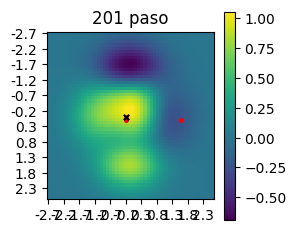
\includegraphics[width=\textwidth]{p7p_200.png}
         \caption{}
         \label{fig:tocan}
     \end{subfigure}
     \begin{subfigure}[b]{0.40\textwidth}
         \centering
         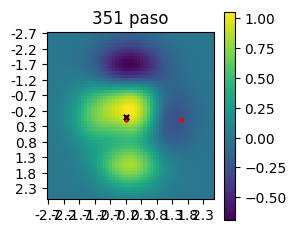
\includegraphics[width=\textwidth]{p7p_350.png}
         \caption{}
         \label{fig:tocan}
         \begin{subfigure}[b]{0.40\textwidth}
         \centering
         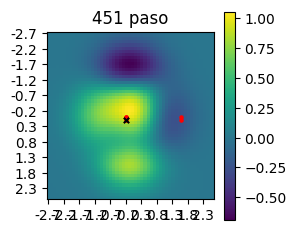
\includegraphics[width=\textwidth]{p7p_450.png}
         \caption{}
         \label{fig:tocan}
     \end{subfigure}
     \end{subfigure}
     \caption{Intervalos de posiciones}
      \label{semilla}
\end{figure}

\newpage

\section{Conclusiones}\label{}
Se concluye que los valores máximos y mínimos de una función con los movimientos aleatorios esto nos da la posición de los puntos que se evaluadas en los vecinos para comparar si es mejor para ser la nueva posición.

\newpage
\section{Reto 1 Cambio de regla del movimiento}\label{}
En este reto consiste en cambiar la regla del movimiento de una solución en X (un vector de dimensión arbitraria) a la siguiente a la de recocido simulado: para optimizar una función \cite{elisa1}. Aquí T es una temperatura que decrece en aquellos pasos donde se acepta una empeora; la reducción se logra multiplicando el valor actual de T. A continuación se muestra en las siguientes instrucciones: 

\begin{lstlisting}[caption=Temperatura, language=Python]
temperatura=100
##temperatura = [100 for i in range(puntos)]
for img in range(ciclos):
    ps,posx,posy,best,temperatura = movimientos(posx, posy, bestx,besty, temperatura)
\end{lstlisting}

Para este reto la vecindad se vuelve a tomar las mismas decisiones, en cada punto inicial que se revisa su vecindad, cada vecindad se selecciona al azar y se remueve en la lista para que el siguiente ciclo no lo toque.
\begin{lstlisting}[caption=Vecindad, language=Python]
vecindad=[(xi,yd),(cx,yd),(xd,yd),(xi,cy),(xd,cy),(xi,yi),(cx,yi),(xd,yi)]
  for k in range(len(vecindad)):
    xnew,ynew = choice(vecindad)
    vecindad.remove((xnew,ynew))
    delta= g(xnew,ynew) - g(cx,cy)
    probabilidad= exp(delta/temp)
    if delta > 0:
    cx, cy=xnew, ynew        
    break
    else:
    if random() < (probabilidad):
    cx, cy=xnew, ynew        
    temp=(temp*(0.995))
    break
    else:
        cx, cy = cx, cy
\end{lstlisting}

\section{Reto 1 Resultados}\label{}
Esto se visualiza el comportamiento de la variación respecto a la temperatura. Se encuentra todos los resultados y gifs en el repositorio \href{https://github.com/satuelisa/Simulation/blob/master/LocalSearch/minimize1D.py}{repositorio} de Nestor en GitHub.\\

\begin{figure}
     \centering
     \begin{subfigure}[b]{0.40\textwidth}
         \centering
         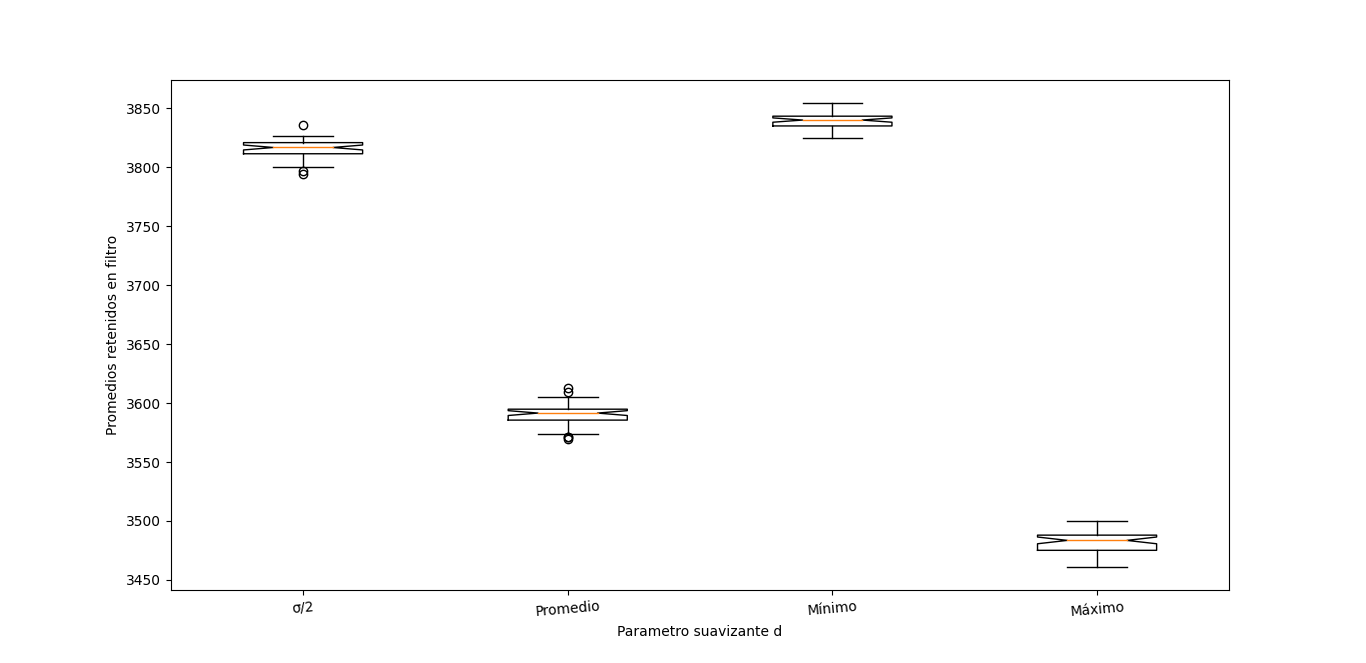
\includegraphics[width=\textwidth]{Figure_1.1.png}
         \caption{}
         \label{fig:notocan}
     \end{subfigure}
     \begin{subfigure}[b]{0.40\textwidth}
         \centering
         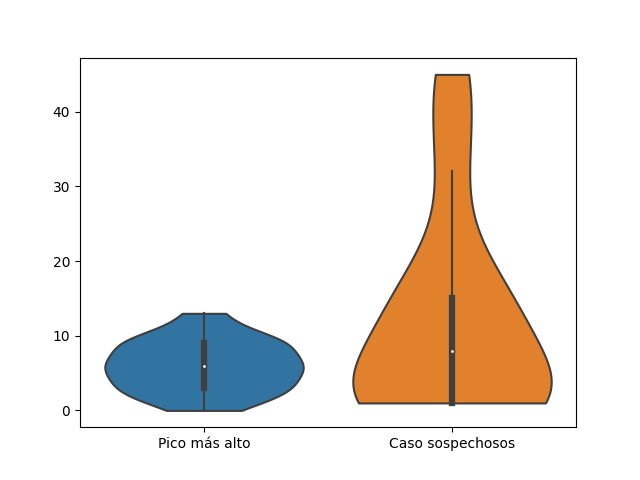
\includegraphics[width=\textwidth]{Figure_2.png}
         \caption{}
         \label{fig:tocan}
     \end{subfigure}
     \begin{subfigure}[b]{0.40\textwidth}
         \centering
         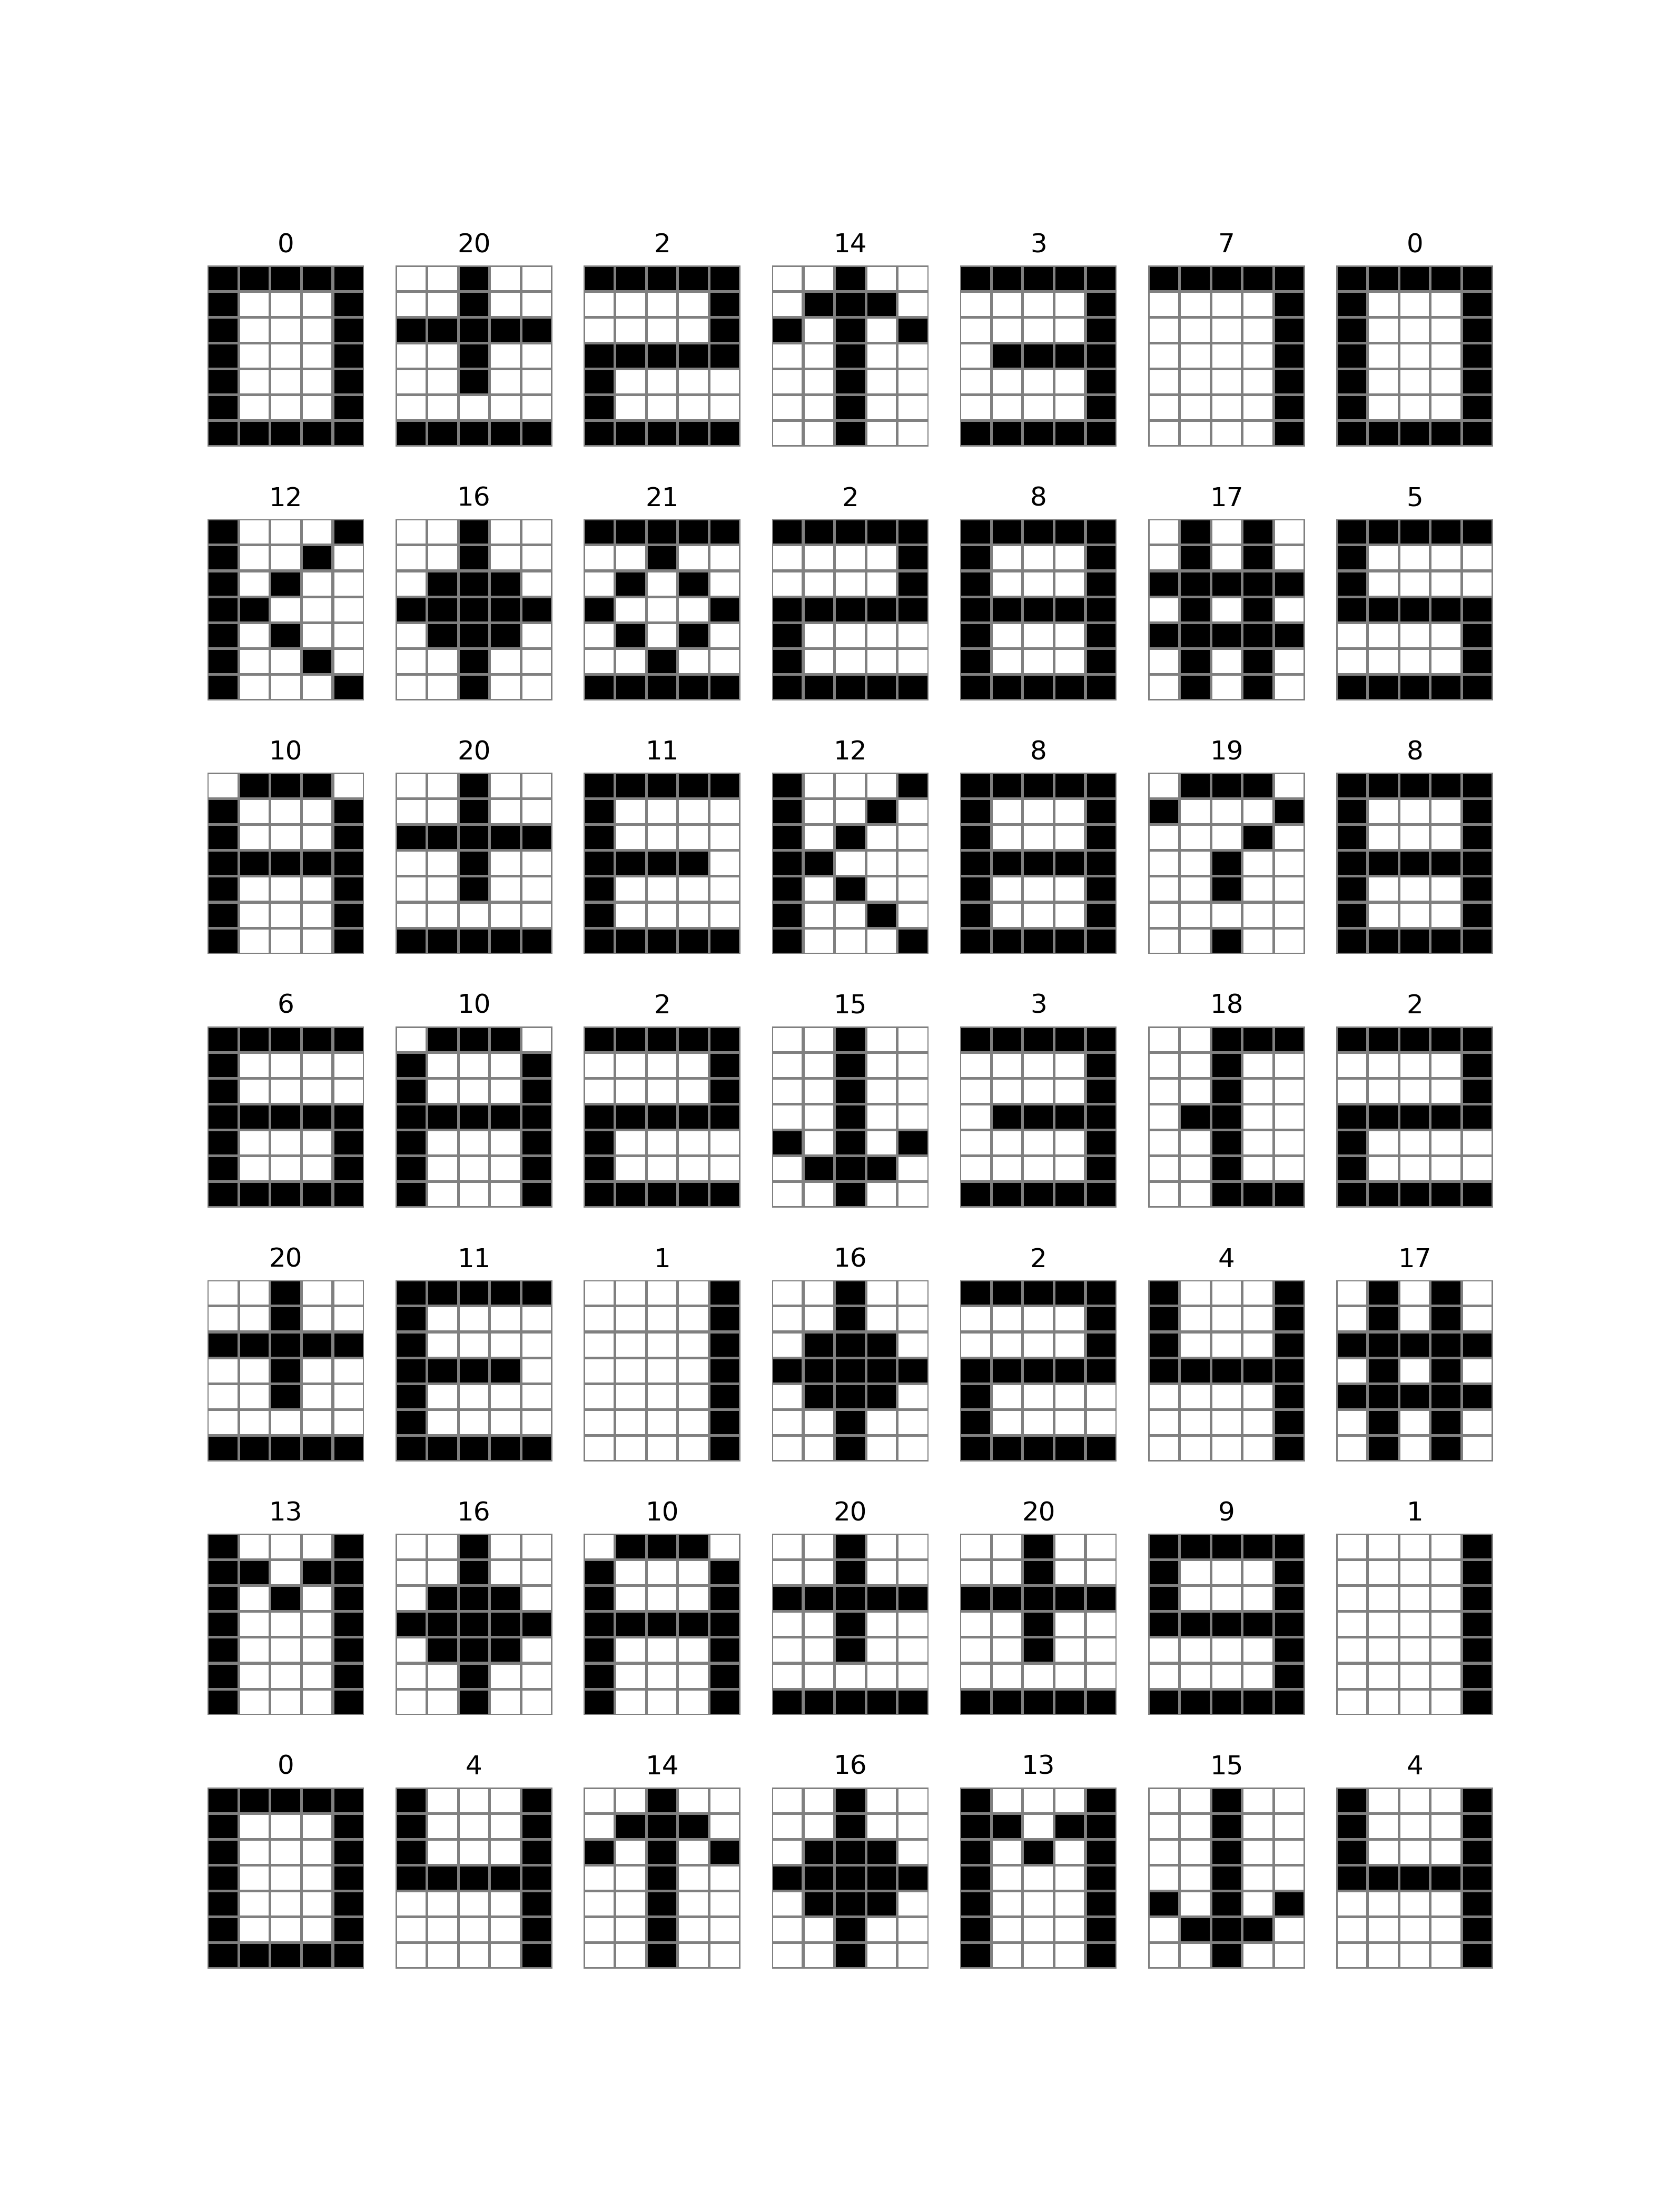
\includegraphics[width=\textwidth]{Figure_3.png}
         \caption{}
         \label{fig:tocan}
     \end{subfigure}
     \begin{subfigure}[b]{0.40\textwidth}
         \centering
         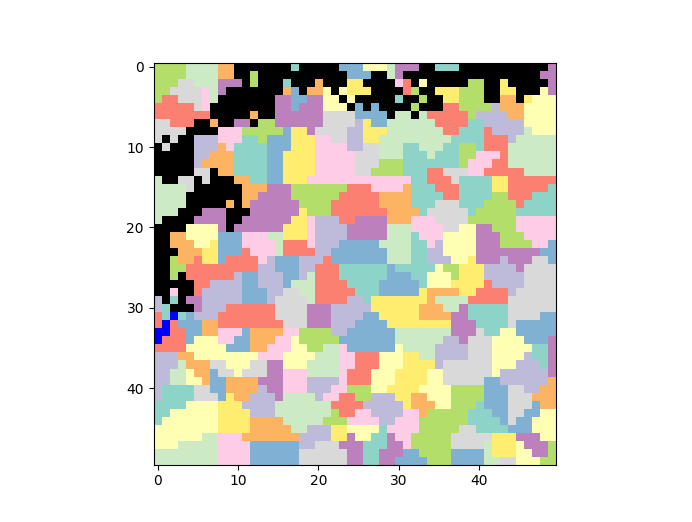
\includegraphics[width=\textwidth]{Figure_4.png}
         \caption{}
         \label{fig:tocan}
         \begin{subfigure}[b]{0.40\textwidth}
         \centering
         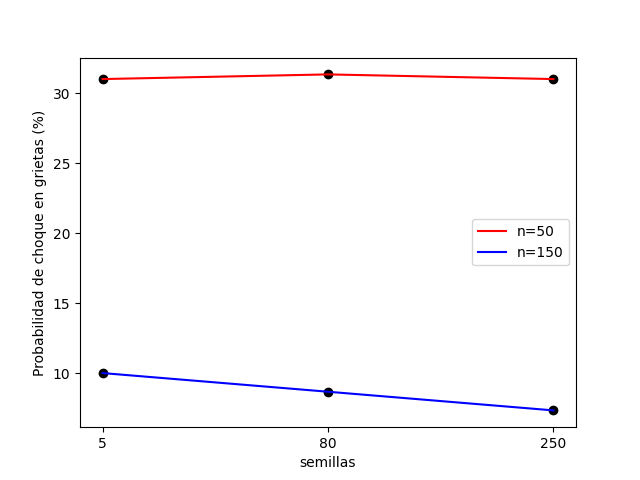
\includegraphics[width=\textwidth]{Figure_5.png}
         \caption{}
         \label{fig:tocan}
     \end{subfigure}
     \end{subfigure}
     \caption{Intervalos de Temperatura}
      \label{semilla}
\end{figure}

\newpage

\section{Reto 2 Comparación de diferencia estadísticamente}\label{}
En este reto consiste en comparar sí o no hay diferencia estadísticamente significativa entre el método de la tarea base y el método del primer reto en términos de la precisión del resultado obtenido (es decir, la diferencia entre el resultado reportado y el óptimo global) en función del número de iteraciones y el número de réplicas \cite{elisa1}. A continuación se muestra en las siguientes instrucciones: 

\begin{lstlisting}[caption=Comparación de iteraciones, language=Python]
iteraciones= (100,500,1000)
CB_est2=[]
for f in iteraciones:
    estimados2=[]
    for r in range(replicas):
        posx = [uniform(low, high) for s in range(puntos)]
        posy = [uniform(low, high)for s in range(puntos)]
        bestx = posx
        besty = posy
        temperatura=1000
        for img in range(f):
            ps,posx,posy,best,temperatura = mov_reto1(posx, posy, bestx,besty, temperatura)
            if img==(f-1):
                mejor=max(best)
                estimados2.append(mejor[0])
    CB_est2.append(estimados2)
plt.boxplot([CB_est2[0], CB_est2[1], CB_est2[2]])
plt.xlabel('iteraciones')
plt.ylabel('Posiciones finales maximizadas')
plt.xticks([1,2,3], ['100','500','1000'])
\end{lstlisting}

\section{Reto 2 Resultados}\label{}
Esto se visualiza la diferencia entre los resultado reportado y la función del número de iteraciones y el número de réplicas estadísticamente. Se encuentra todos los resultados y gifs en el repositorio \href{https://github.com/satuelisa/Simulation/blob/master/LocalSearch/minimize1D.py}{repositorio} de Nestor en GitHub.\\

\newpage
\begin{figure}
    \centering
    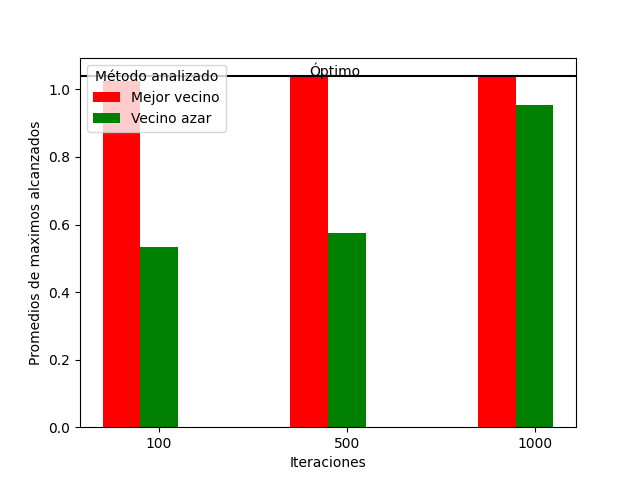
\includegraphics[width=200mm]{comparacion_metodos.png}
    \caption{Diagrama de comparación de iteraciones}
    \label{figure}
\end{figure}

\begin{figure}
    \centering
    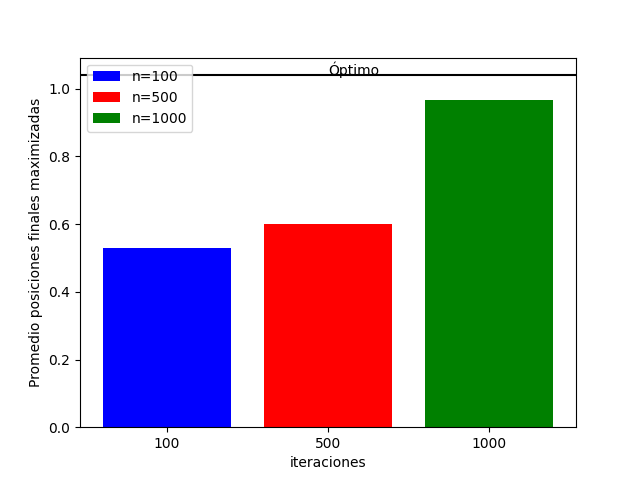
\includegraphics[width=200mm]{R1_prom_vec_azar.png}
    \caption{Diagrama promedio de posiciones de vecinos al azar}
    \label{figure}
\end{figure}

\begin{figure}
    \centering
    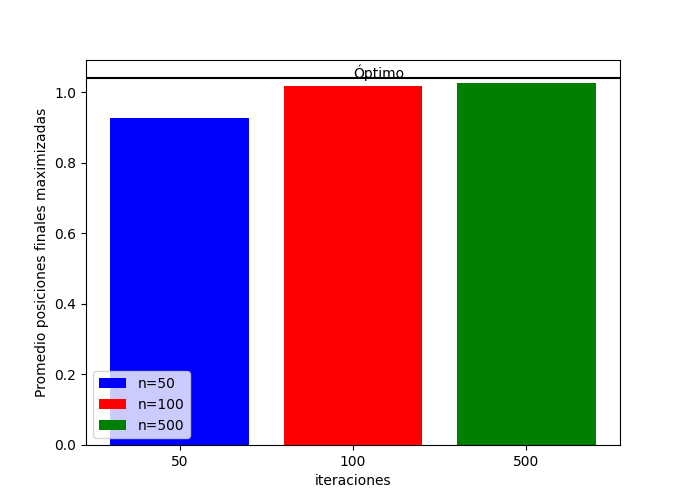
\includegraphics[width=200mm]{R1_prom_vec_max.png}
    \caption{Diagrama promedio de posiciones de vecinos máximos}
    \label{figure}
\end{figure}

\begin{figure}
    \centering
    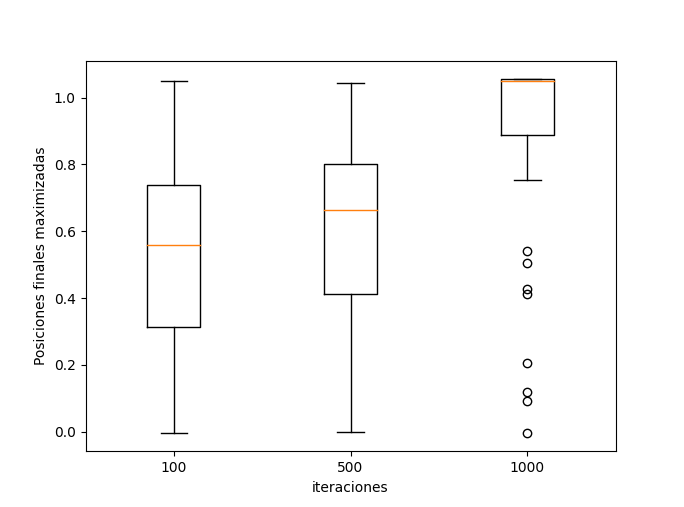
\includegraphics[width=200mm]{R1_vecinos_azar.png}
    \caption{Diagrama de vecinos al azar}
    \label{figure}
\end{figure}

\begin{figure}
    \centering
    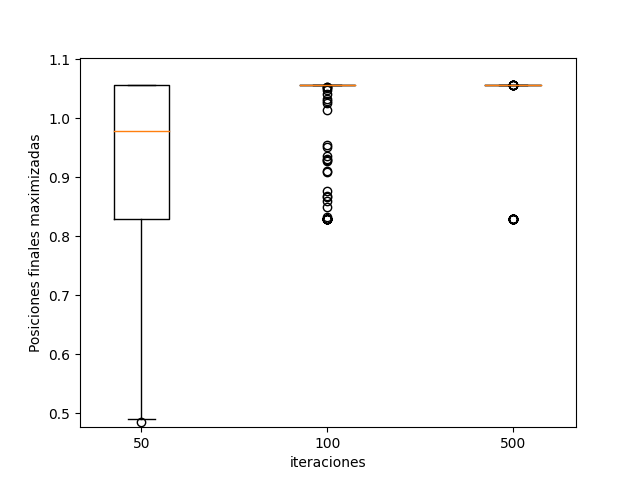
\includegraphics[width=200mm]{R1_vecinos_max.png}
    \caption{Diagrama de vecinos máximos}
    \label{figure}
\end{figure}

\bibliographystyle{plainnat}
\bibliography{simulacion}
\end{document}
